\begin{figure}[ht]
\begin{center}
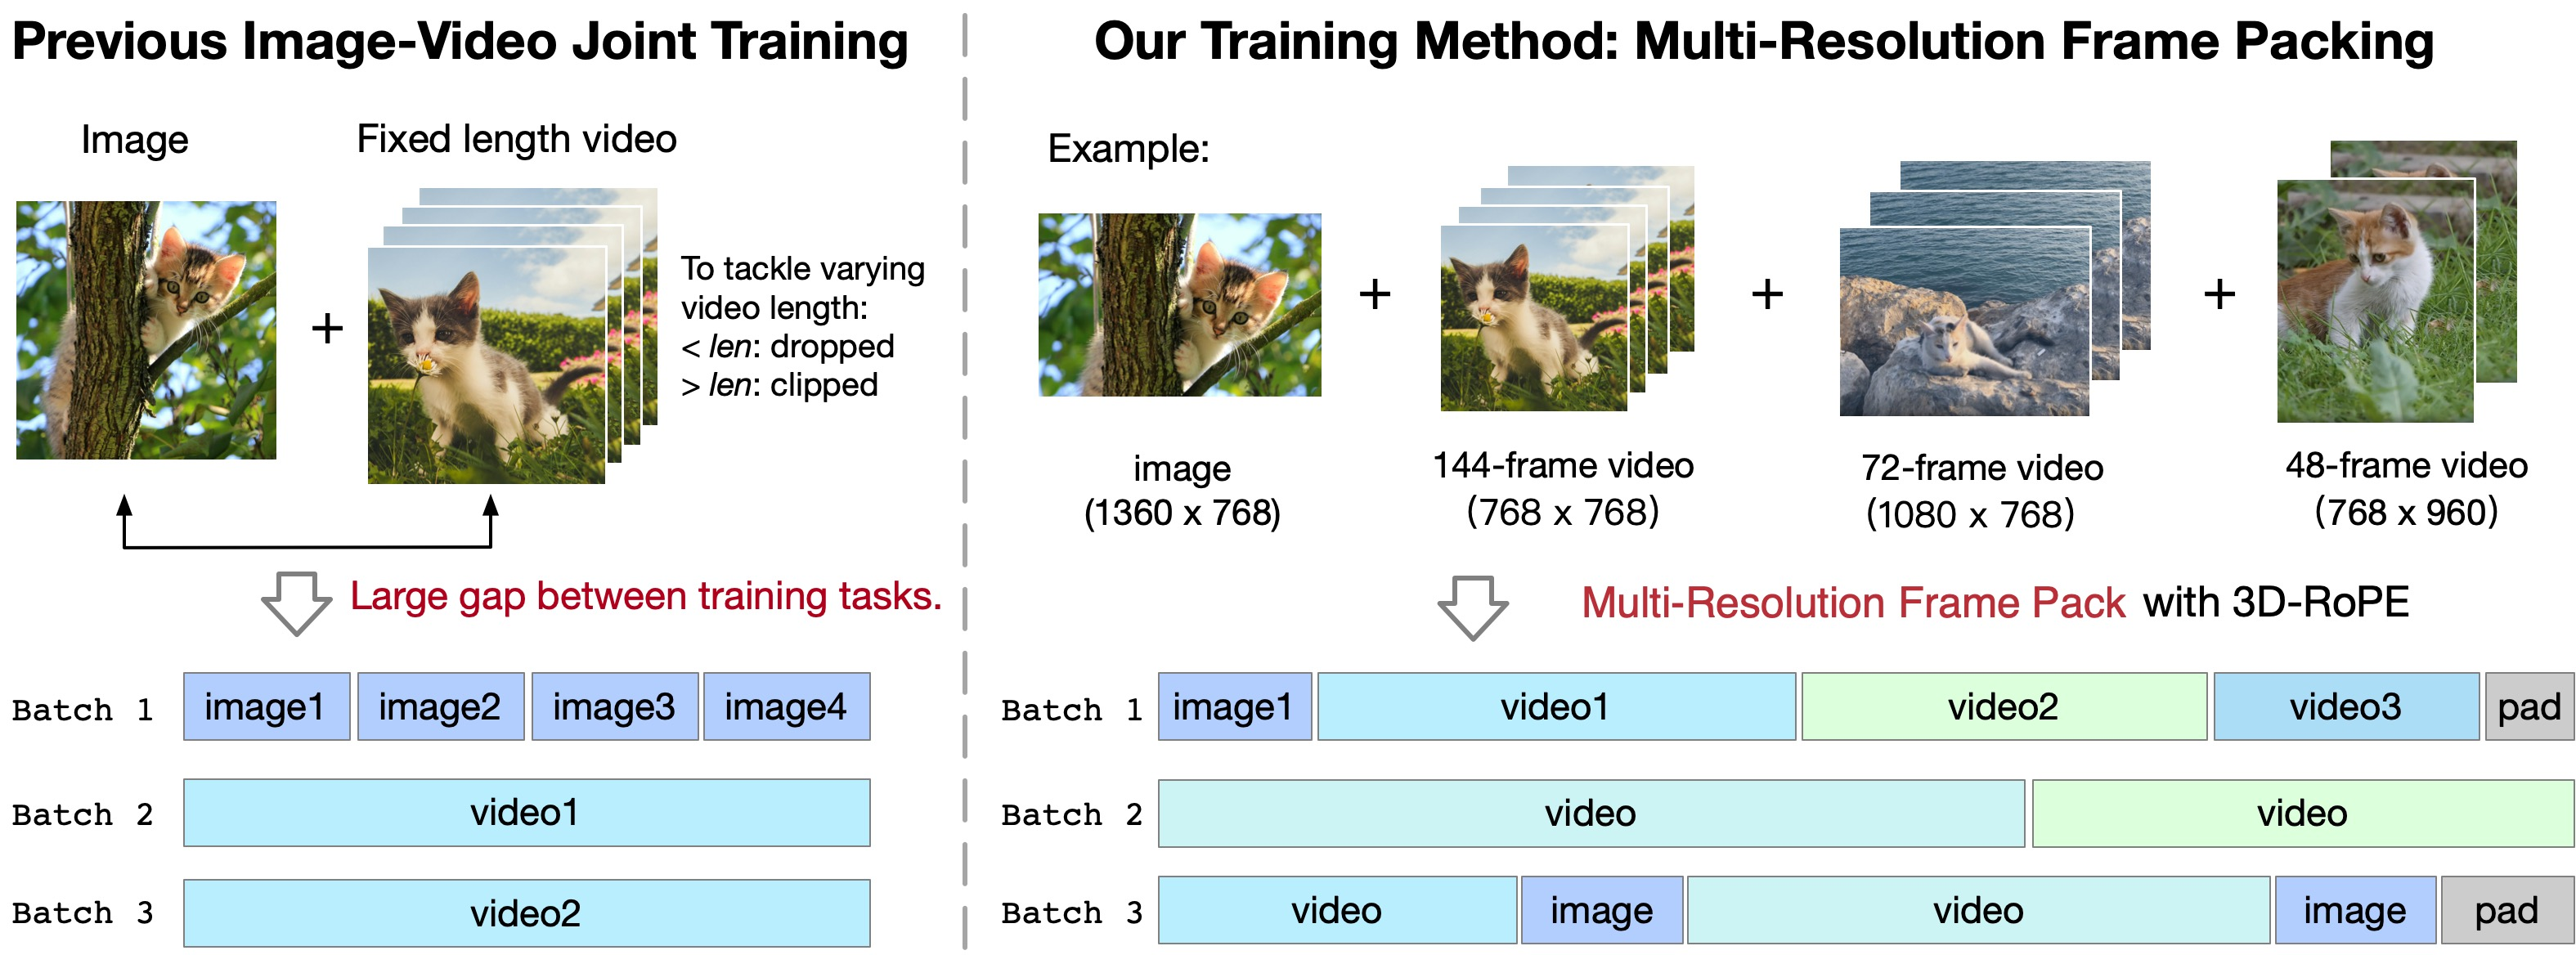
\includegraphics[width=\linewidth]{images/CogVideoX-framepacking-2.jpg}
\end{center}
\caption{
The diagram of mixed-duration training and Frame Pack. To fully utilize the data and enhance the model's generalization capability, we train on videos of different duration within the same batch.}
\label{fig:framepack}
\vspace{-5mm}
\end{figure}

\section{Training \model}

%\subsection{Setting}
We mix images and videos during training, treating each image as a single-frame video. 
Additionally, we employ progressive training from the resolution perspective. 
For the diffusion setting, we adopt v-prediction~\citep{salimans2022progressive} and zero SNR~\citep{lin2024common}, following the noise schedule used in LDM~\citep{rombach2022high}.

\subsection{Multi-Resolution Frame Pack}
Previous video training methods often involve joint training of images and videos with a fixed number of frames~\citep{singer2022make, blattmann2023stable}. 
However, this approach usually leads to two issues: 
First, there is a significant gap between the two input types using bidirectional attention, with images having one frame while videos having dozens of frames. 
We observe that models trained this way tend to diverge into two generative modes based on the token count and not to have good generalizations. %e well. 
Second, to train with a fixed duration, we have to discard short videos and truncate long videos, which prevents full utilization of the videos of varying number of frames.

To address these issues, we choose mixed-duration training, which means training videos of different lengths together. 
However, inconsistent data shapes within the batch make training difficult. 
Inspired by Patch'n Pack \citep{dehghani2024patch}, we place videos of different duration (also in different resolutions) into the same batch to ensure consistent shapes within each batch, a method we refer to as \textit{Multi-Resolution Frame Pack}. The process is illustrated in Figure~\ref{fig:framepack}. 

We use 3D RoPE to model the position relationship of various video shape. There are two ways to adapt RoPE to different resolutions and durations. One approach is to expand the position encoding table and, for each video, select the front portion of the table according to the resolution (extrapolation). The other is to scale a fixed-length position encoding table to match the resolution of the video (interpolation). Considering that RoPE is a relative position encoding, we chose the first approach to keep the clarity of model details.


\subsection{Progressive Training}
Videos from the Internet usually include a significant amount of low-resolution ones. And directly training on high-resolution videos is extremely expensive. To fully utilize data and save costs, the model is first trained on 256px videos to learn semantic and low-frequency knowledge. Then it is trained on gradually increased resolutions, from 256px to 512px, 768px, to learn high-frequency knowledge. To maintain the ability of generating videos with different aspect ratios, we keep the aspect ratio unchanged and resize the short side to above resolutions. Finally, we select a subset of high-quality videos to fine-tune the model, since the filtered pre-training data still contains a certain proportion of dirty data, such as subtitles, watermarks, and low-bitrate videos. We find this step can effectively remove generated subtitles and watermarks and improve the visual quality.
Moreover, we trained an image-to-video model based on above model. See Appendix~\ref{app:i2v} for details.
 
% (\tjy:)The training pipeline of \model is divided into three stages: low-resolution training, high-resolution training, and high-quality video fine-tuning. 
% Similar to images, videos from the Internet usually include a significant amount of low-resolution ones. 
% Progressive training can effectively utilize videos of various resolutions. 
% Moreover, training at low resolution initially can equip the model with coarse-grained modeling capabilities, followed by high-resolution training to enhance its ability to capture fine details. 
% Compared to direct high-resolution training, staged training can also help reduce the overall training time.

% \begin{figure}[h]
% \begin{center}
% 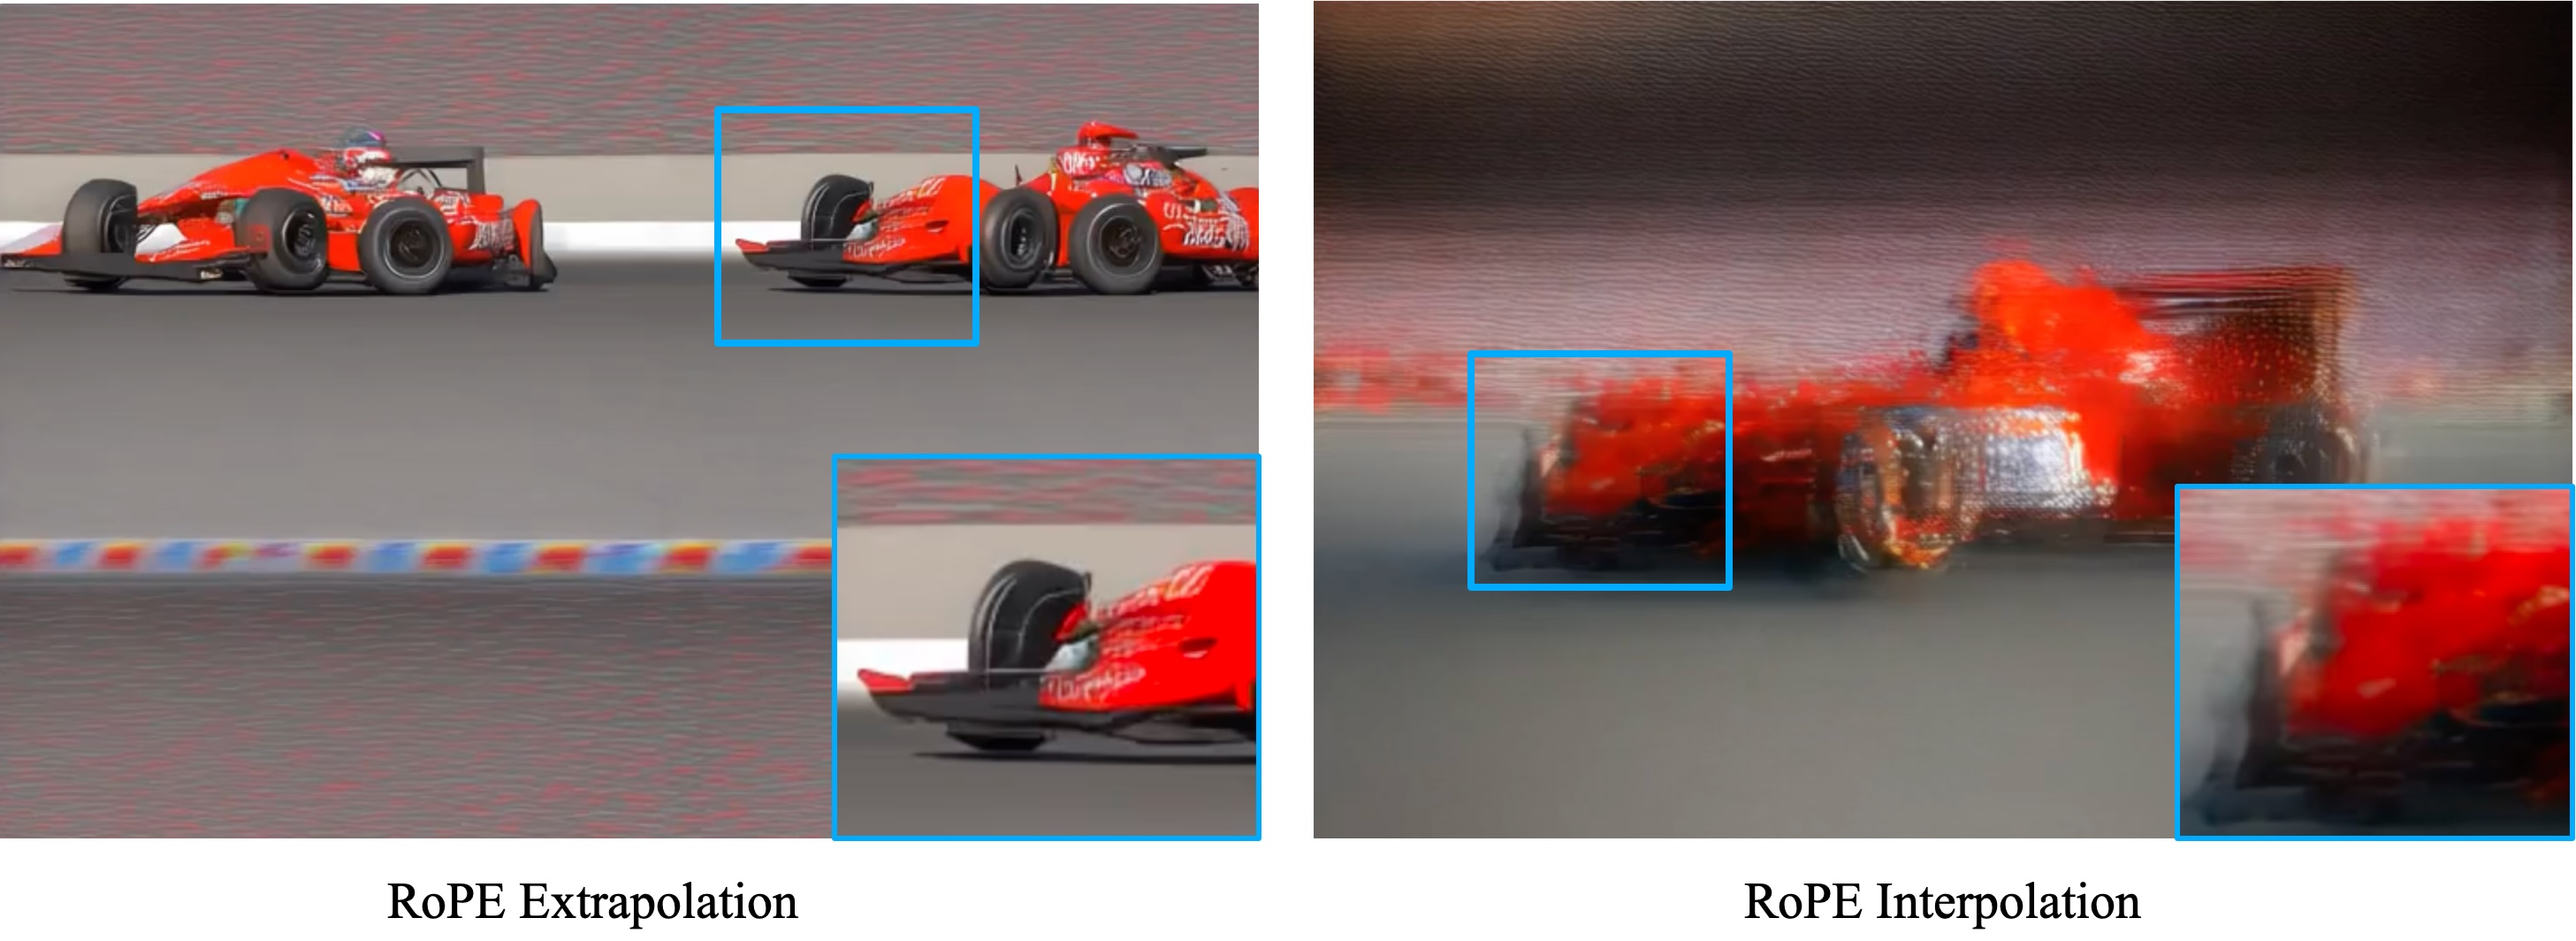
\includegraphics[width=0.9\linewidth]{images/ive.jpg}
% \end{center}
% \caption{The comparison between the initial generation states of extrapolation and interpolation when increasing the resolution with RoPE encoding. Extrapolation tends to generate multiple small, clear, and repetitive images, while interpolation generates a blurry large image.}
% \label{fig:ive}
% \end{figure}

% \paragraph{Extrapolation of Position Code.}
% When adapting low-resolution position encoding to high-resolution, we consider two different methods: interpolation and extrapolation. We show the effects of two methods in Figure~\ref{fig:ive}. Interpolation tends to preserve global information more effectively, whereas the extrapolation better retains local details. Given that RoPE is a relative position encoding, We chose the extrapolation to maintain the relative position between pixels. 

% \paragraph{High-Quality Fine-Tuning.}
% Since the filtered pre-training data still contains a certain proportion of dirty data, such as subtitles, watermarks, and low-bitrate videos, we selected a subset of higher quality video data, accounting for 20\% of the total dataset, for fine-tuning in the final stage. This step effectively removed generated subtitles and watermarks and slightly improved the visual quality. However, we also observed a slight degradation in the model's semantic ability.


\subsection{Explicit Uniform Sampling}

~\citet{ho2020denoising} defines the training objective of diffusion as 
\begin{equation}~\label{eq:ddpm-loss}
    L_\mathrm{simple}(\theta) := \mathbf{E}_{t, x_0, \epsilon}{ \left\| \epsilon - \epsilon_\theta(\sqrt{\bar\alpha_t} x_0 + \sqrt{1-\bar\alpha_t}\epsilon, t) \right\|^2},
\end{equation}
where $t$ is uniformly distributed between 1 and T. 
The common practice is for each rank in the data parallel group to uniformly sample a value between 1 and $T$, which is in theory equivalent to Equation~\ref{eq:ddpm-loss}. 
However, in practice, the results obtained from such random sampling are often not sufficiently uniform, and since the magnitude of the diffusion loss is related to the timesteps, this can lead to significant fluctuations in the loss. 
Thus, we propose to use \textit{Explicit Uniform Sampling} to divide the range from 1 to $T$ into $n$ intervals, where $n$ is the number of ranks. 
Each rank then uniformly samples within its respective interval. 
This method ensures a more uniform distribution of timesteps. 
As shown in Figure~\ref{fig:subfigures} (d), the loss curve from training with Explicit Uniform Sampling is noticeably more stable. 

In addition, we compare the loss at each diffusion timestep alone between two choices for a more precise comparison. We find after using explicit uniform sampling, the loss at all timesteps decreased faster, indicating that this method can also accelerate loss convergence.